\documentclass{standalone}
\usepackage{tikz}
\usepackage{fontspec}
\usetikzlibrary{matrix}

% Set up Bengali font (use any Bengali font installed on your system)
\newfontfamily\bengalifont{Noto Sans Bengali}[Script=Bengali]

\begin{document}
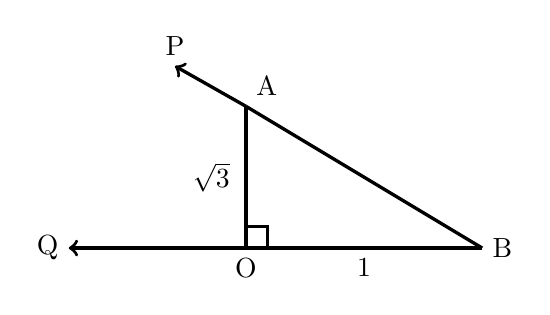
\begin{tikzpicture}[scale=1.5, thick]
    % Define coordinates
    \coordinate (O) at (0,0);
    \coordinate (Q) at (-1.5,0);
    \coordinate (B) at (2,0);
    \coordinate (A) at (0,1.2);
    \coordinate (P) at (-0.6,1.54);
    
    % Draw horizontal line with arrow on left
    \draw[->][very thick] (O) -- (Q);
    \draw[very thick] (O) -- (B);
    
    % Draw vertical line OA
    \draw[very thick] (O) -- (A);
    
    % Draw line from P through A to B
    \draw[->][very thick] (A) -- (P);
    \draw[very thick] (A) -- (B);
    
    % Draw right angle at O
    \draw[very thick] (0,0.18) -- (0.18,0.18) -- (0.18,0);
    
    % Labels
    \node[above] at (P) {P};
    \node[above right] at (A) {A};
    \node[left] at (Q) {Q};
    \node[below] at (O) {O};
    \node[right] at (B) {B};
    
    % Measurements
    \node[left] at (-0.05,0.6) {$\sqrt{3}$};
    \node[below] at (1,0) {$1$};
\end{tikzpicture}
\end{document}